\documentclass[preprint,12pt]{elsarticle}

% -------------------------------------------------------------------------
% Packages
% -------------------------------------------------------------------------
\usepackage[utf8]{inputenc}
\usepackage[T1]{fontenc}
\usepackage{amsmath}
\usepackage{amssymb}
\usepackage{tikz}
\usepackage{textcomp}
\usepackage{multirow}
\usepackage{float}
\usepackage{booktabs}
\usepackage{tabularx}
\usepackage{array}
\usepackage{pgfplots}
\usepackage{pgfplotstable}
\usepackage{siunitx}
\usepackage{xcolor}
\usepackage{enumitem}
\usepackage{url}

\pgfplotsset{compat=1.18}
\usetikzlibrary{
    arrows.meta,
    positioning,
    calc,
    shapes.geometric,
    fit,
    backgrounds,
    decorations.pathmorphing
}

% -------------------------------------------------------------------------
% TikZ styles
% -------------------------------------------------------------------------
\tikzset{
    blockblue/.style={
        draw=blue!55!black,
        fill=blue!8,
        rounded corners=2pt,
        thick,
        align=center,
        minimum height=0.85cm,
        text width=3.1cm,
        font=\footnotesize
    },
    blockgreen/.style={
        draw=green!45!black,
        fill=green!8,
        rounded corners=2pt,
        thick,
        align=center,
        minimum height=0.85cm,
        text width=3.1cm,
        font=\footnotesize
    },
    blockorange/.style={
        draw=orange!70!black,
        fill=orange!12,
        rounded corners=2pt,
        thick,
        align=center,
        minimum height=0.85cm,
        text width=3.1cm,
        font=\footnotesize
    },
    blockred/.style={
        draw=red!60!black,
        fill=red!8,
        rounded corners=2pt,
        thick,
        align=center,
        minimum height=0.85cm,
        text width=3.1cm,
        font=\footnotesize
    },
    arrow/.style={
        -{Latex[length=2mm]},
        thick
    },
    station/.style={
        dashed,
        thick,
        gray
    }
}

% -------------------------------------------------------------------------
% Document
% -------------------------------------------------------------------------
\begin{document}

\begin{frontmatter}

\title{One-Dimensional Numerical Modelling of a Supersonic RAMJET Engine with Parametrizable Geometry}

% Authors and Affiliations
\author[1]{Santiago Cadavid Franco\corref{cor1}}
\ead{santiago.cadavid@javeriana.edu.co}

\author[1]{Camilo Bayona Roa}
\ead{camilo.bayona@javeriana.edu.co}

\cortext[cor1]{Corresponding author}

\address[1]{Department of Industrial Engineering, Pontificia Universidad Javeriana, Bogotá, Colombia}

\begin{abstract}
This article presents a one-dimensional numerical model of a supersonic RAMJET engine with parametrizable geometry. The model was developed to reproduce the main aero-thermodynamic behavior of the engine using a reduced-order computational approach suitable for preliminary design, geometric sensitivity, and fast simulation studies. The methodology combines compressible-flow relations, a parametrized axial geometry, the area--velocity equation, a simplified combustion energy balance, the sonic condition at the nozzle throat, and the expansion process in a convergent-divergent nozzle. The geometry is defined through axial functions for the external duct radius and the internal spike radius, from which the effective annular flow area and its spatial derivative are obtained. Cubic Hermite interpolation is used to construct smooth geometric profiles and continuous area gradients. The model was implemented in MATLAB and evaluated under a baseline supersonic operating condition. The results reproduce the expected physical sequence of a RAMJET engine: aerodynamic compression, heat addition, choked flow at the throat, supersonic expansion, and positive net thrust generation. The baseline simulation produced a net thrust of 1719.4 N, a specific impulse of 2094.6 s, an exit Mach number of 2.033, and a global efficiency of 30.3\%. In addition, a sensitivity analysis was conducted to identify the influence of flight Mach number, post-inlet Mach number, inlet radius, fuel-to-air ratio, and pressure recovery factors on net thrust. The proposed methodology provides a low-cost computational tool for analyzing the influence of geometry and operating conditions on RAMJET performance and can serve as a basis for future optimization and higher-fidelity validation studies.
\end{abstract}

\begin{keyword}
RAMJET engine \sep one-dimensional model \sep supersonic propulsion \sep parametrizable geometry \sep compressible flow \sep MATLAB \sep numerical simulation \sep thrust \sep sensitivity analysis
\end{keyword}

\end{frontmatter}

% =========================================================================
\section{Introduction}
\label{sec:introduction}
% =========================================================================
% =========================================================================
Supersonic propulsion remains one of the most relevant fields in aerospace engineering due to its potential applications in high-speed vehicles, defense systems, unmanned aerial platforms, and atmospheric or suborbital exploration missions. Within this context, RAMJET engines represent a relevant alternative for supersonic flight regimes, since they do not require compressors or turbines to increase the pressure of the incoming flow. Instead of relying on turbomachinery, this type of engine uses the high flight speed of the vehicle and the geometric configuration of its inlet to decelerate the air, increase its pressure and temperature, add energy through combustion, and subsequently expand the hot gases through a convergent-divergent nozzle to generate thrust \cite{Hill1992,Mattingly2006,NASA2015}.
Despite their apparent mechanical simplicity, the internal behavior of a RAMJET engine is highly dependent on the interaction between duct geometry and compressible flow. The supersonic inlet, the central body or \textit{spike}, the diffuser, the combustion chamber, and the nozzle must operate in a coupled manner to ensure adequate aerodynamic compression, stable combustion, and efficient expansion. Consequently, small variations in the effective flow area may significantly modify the evolution of the Mach number, pressure, temperature, density, and flow velocity along the engine \cite{Anderson1990,Heiser1994}.
The analysis of this type of propulsion system involves several challenges. On the one hand, access to real RAMJET engine geometries is usually limited due to their specialized nature and restricted applications. On the other hand, high-fidelity simulations based on computational fluid dynamics require a detailed geometric description, mesh generation, significant computational resources, and long processing times. These conditions make it difficult to rapidly explore multiple geometric configurations during preliminary design stages. For this reason, low-dimensional and reduced-order models constitute a useful alternative for studying the overall behavior of propulsion systems, provided that they preserve the fundamental physical principles governing the flow \cite{Bayona2019,Burden2011}.
Previous computational studies on RAMJET-type engines have focused on thermodynamic cycle analysis, fuel comparison, and performance estimation under different supersonic operating conditions \cite{Dallos2024}. However, one of the main limitations in preliminary RAMJET analysis is the difficulty of linking the geometry of the inlet, spike, chamber, throat, and nozzle with the internal evolution of the flow in a simple and reproducible computational framework. This limitation is especially relevant because the area distribution and its derivative directly influence the behavior of compressible flow through the area--velocity relation \cite{Anderson1990,Mattingly2006}.
In this work, a one-dimensional numerical model of a supersonic RAMJET engine with parametrizable geometry is developed and implemented in MATLAB. The model integrates the geometric definition of the engine, compressible-flow relations, the area--velocity equation, the energy balance in the combustion chamber, the sonic condition at the throat, and the expansion process in a convergent-divergent nozzle. The geometry is not introduced as a static figure, but as a set of functions dependent on the axial coordinate, from which the effective flow area and its spatial derivative are computed \cite{Cadavid2025}.
The main contribution of this article is the presentation of a reproducible computational methodology to reconstruct and evaluate the RAMJET model in a simulation environment. To this end, the input variables, model assumptions, geometric parametrization, nodal discretization, governing equations, and numerical procedure used to compute the Mach number, velocity, pressure, temperature, density, and area profiles along the engine are described.
The article is organized as follows. Section~\ref{sec:physical_description} describes the physical architecture of the RAMJET engine and the main assumptions of the model. Section~\ref{sec:mathematical_formulation} presents the mathematical formulation of the flow, combustion, expansion, and performance calculations. Section~\ref{sec:numerical_implementation} presents the parametric geometry and numerical implementation. Section~\ref{sec:results} presents the baseline case results and sensitivity analysis. Finally, Section~\ref{sec:conclusions} summarizes the main conclusions, limitations, and possible directions for future work.
% =========================================================================
\section{Physical Description of the RAMJET Engine}
\label{sec:physical_description}
% =========================================================================
The RAMJET engine considered in this work is modeled as an air-breathing propulsion system operating under supersonic flight conditions. Unlike conventional turbojet or turbofan engines, the RAMJET does not include compressors, turbines, or rotating machinery. Instead, the compression process is achieved aerodynamically by using the kinetic energy of the incoming supersonic flow and the internal geometry of the engine \cite{Hill1992,Mattingly2006}.
The engine is interpreted according to the main processes of the Brayton cycle: compression, heat addition, and expansion. In the first stage, the incoming air enters the engine at a supersonic Mach number and is progressively decelerated through the inlet, spike, and diffuser. This controlled deceleration converts part of the kinetic energy of the flow into static pressure and temperature, preparing the air for combustion. In the second stage, fuel is added to the compressed air inside the combustion chamber, increasing the total thermal energy of the flow. Finally, the hot combustion gases are expanded through a convergent-divergent nozzle, where thermal and pressure energy are converted into kinetic energy to generate thrust \cite{Hill1992,Mattingly2006,Heiser1994}.
\subsection{Engine Architecture and Functional Zones}
The RAMJET geometry is represented as an axisymmetric duct composed of an external casing and an internal body associated with the spike. This configuration defines an annular flow passage whose effective area varies along the axial coordinate. The engine domain is divided into a set of characteristic stations that identify the boundaries between the main physical regions of the model:
\begin{equation}
x_a,\; x_0,\; x_1,\; x_2,\; x_3,\; x_4,\; x_5,\; x_6 .
\end{equation}
The station $x_a$ represents the free-stream condition upstream of the engine. The station $x_0$ corresponds to the inlet reference plane, where the captured flow begins to be processed by the internal geometry. The interval from $x_0$ to $x_2$ represents the aerodynamic compression region, including the inlet, spike, and diffuser. The combustion chamber is located between $x_2$ and $x_4$. The station $x_5$ corresponds to the nozzle throat, and $x_6$ represents the nozzle exit.
\begin{figure}[H]
\centering
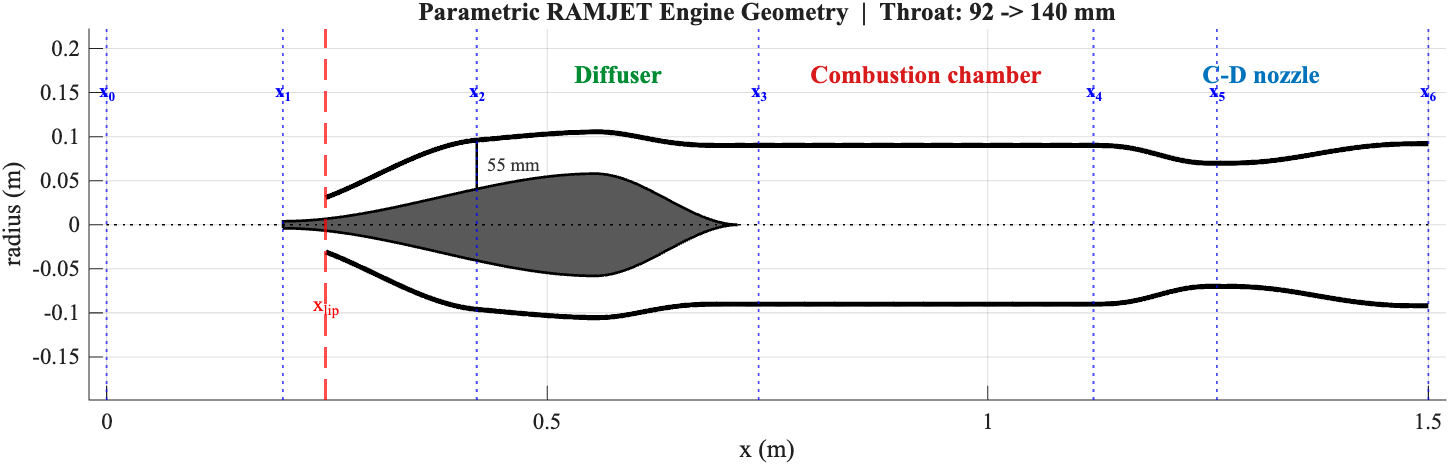
\includegraphics[width=1.2\textwidth]{RAMJET Geometry.png}
\caption{Parametric RAMJET geometry generated in MATLAB. The figure shows the external duct radius, internal spike radius, annular flow region, and main thermodynamic stations used in the numerical model.}
\label{fig:ramjet_geometry_matlab}
\end{figure}
\subsection{Operating Variables}
The operating variables define the flight condition, atmospheric state, fuel addition, and efficiency factors used to represent internal losses. These variables are summarized in Table~\ref{tab:ramjet_operating_variables}.
\begin{table}[H]
\centering
\caption{Main operating variables used in the RAMJET model.}
\label{tab:ramjet_operating_variables}
\begin{tabularx}{\textwidth}{lll}
\toprule
\textbf{Variable} & \textbf{Symbol} & \textbf{Role in the model} \\
\midrule
Flight Mach number & $M_a$ & Defines the supersonic inlet regime \\
Ambient temperature & $T_a$ & Defines the initial thermal state and speed of sound \\
Ambient pressure & $P_a$ & Defines the free-stream pressure reference \\
Ambient density & $\rho_a$ & Used to compute captured mass flow \\
Flight velocity & $u_a$ & Represents the initial axial flow velocity \\
Air mass flow rate & $\dot{m}_a$ & Determines the available air for combustion \\
Fuel-to-air ratio & $f$ & Controls the energy added during combustion \\
Fuel mass flow rate & $\dot{m}_f$ & Defines the injected fuel mass flow \\
Lower heating value & LHV & Represents the chemical energy of the fuel \\
Combustion efficiency & $\eta_b$ & Corrects the useful heat released in the chamber \\
Inlet pressure recovery & $\eta_d$ & Represents total pressure losses in the inlet system \\
Combustor pressure ratio & $\sigma_b$ & Represents pressure losses during combustion \\
\bottomrule
\end{tabularx}
\end{table}
\subsection{Modeling Assumptions and Scope}
The model is developed as a one-dimensional and steady-state representation of the internal flow. Thus, all flow properties are considered functions of the axial coordinate $x$, while temporal variations and three-dimensional effects are not explicitly resolved. This assumption is commonly used in preliminary propulsion analysis when the objective is to evaluate global behavior with reduced computational cost \cite{Hill1992,Mattingly2006}.
The working fluid is treated as a perfect gas with constant thermodynamic properties. The compression process is modeled through compressible-flow relations coupled with the area variation of the duct. The combustion chamber is represented through a simplified energy balance with a prescribed fuel-to-air ratio, combustion efficiency, and pressure loss factor. The nozzle is modeled as a convergent-divergent duct in which the sonic condition is imposed at the throat and the flow is subsequently expanded toward the exit section.
% =========================================================================
\section{Mathematical Formulation of the RAMJET Model}
\label{sec:mathematical_formulation}
% =========================================================================
The mathematical formulation of the RAMJET model is based on a one-dimensional representation of compressible flow along the engine axis. The objective of this formulation is to compute the evolution of the main flow variables from the free-stream condition to the nozzle exit, considering aerodynamic compression, heat addition, expansion, and global propulsion performance. The governing relations are based on standard compressible-flow theory and gas-turbine propulsion analysis \cite{Anderson1990,Hill1992,Mattingly2006}.
The model computes the axial distribution of the Mach number, velocity, static temperature, static pressure, density, and effective flow area:
\begin{equation}
M(x),\; u(x),\; T(x),\; P(x),\; \rho(x),\; A(x).
\end{equation}
\subsection{Compressible-Flow Relations}
The working fluid is modeled as a perfect gas. Therefore, the static pressure, density, and temperature are related by the ideal gas equation:
\begin{equation}
P = \rho R T,
\end{equation}
where $R$ is the specific gas constant.
The local speed of sound is calculated as
\begin{equation}
c(x)=\sqrt{\gamma R T(x)},
\end{equation}
where $\gamma$ is the specific heat ratio. The local Mach number is then defined as
\begin{equation}
M(x)=\frac{u(x)}{c(x)}
=\frac{u(x)}{\sqrt{\gamma R T(x)}}.
\end{equation}
\subsection{Inlet and Free-Stream Conditions}
Given the flight Mach number $M_a$, ambient temperature $T_a$, and ambient pressure $P_a$, the free-stream velocity is computed as
\begin{equation}
u_a = M_a \sqrt{\gamma R T_a}.
\end{equation}
The ambient density is obtained from the perfect gas relation:
\begin{equation}
\rho_a = \frac{P_a}{R T_a}.
\end{equation}
The captured air mass flow rate is calculated as
\begin{equation}
\dot{m}_a = \rho_a u_a A_a,
\end{equation}
where $A_a$ is the effective capture area at the inlet.
\subsection{Aerodynamic Compression Model}
The aerodynamic compression process is the first physical mechanism that allows the RAMJET engine to operate without rotating compressors. In this region, the incoming supersonic flow is progressively decelerated by the inlet, spike, and diffuser geometry. This deceleration converts part of the kinetic energy of the flow into static pressure and temperature, preparing the air for combustion.
The most important differential equation used in the present model is the area--velocity relation:
\begin{equation}
\frac{du}{dx}
=
\frac{u}{M^2-1}
\frac{1}{A}
\frac{dA}{dx}.
\label{eq:area_velocity}
\end{equation}
This relation is a classical result of quasi-one-dimensional compressible-flow theory and is fundamental for understanding the opposite response of subsonic and supersonic flows to area variation \cite{Anderson1990}. In the present model, Equation~\eqref{eq:area_velocity} constitutes the main coupling between the parametrized geometry and the internal flow solution. The term $A(x)$ represents the effective annular flow area, while $dA/dx$ represents the axial variation of that area. Therefore, any modification in the inlet, spike, diffuser, chamber, throat, or nozzle geometry changes $A(x)$ and $dA/dx$, and consequently modifies the axial velocity field $u(x)$.
The importance of Equation~\eqref{eq:area_velocity} is that it determines how the flow responds to a geometric contraction or expansion depending on the local Mach number. For subsonic flow, an increase in area tends to decelerate the flow, while a decrease in area tends to accelerate it. For supersonic flow, the opposite behavior occurs: an increase in area accelerates the flow, while a decrease in area decelerates it. This change of behavior is governed by the denominator $M^2-1$, which makes the Mach number a critical variable throughout the simulation.
For this reason, the correct management of the Mach number in each region of the engine is fundamental. At the inlet, the flow enters at supersonic conditions and must be compressed aerodynamically. Before combustion, the Mach number must be sufficiently reduced to allow a physically consistent heat-addition process. At the nozzle throat, the flow must reach the sonic condition, $M=1$, which defines the critical section of the convergent-divergent nozzle. Downstream of the throat, the divergent nozzle must accelerate the gases again toward supersonic exit conditions. Thus, the Mach number is not only an output variable, but also a physical indicator that determines whether each section of the engine is operating consistently.
During the compression process, no heat addition or external mechanical work is considered. Thus, the total temperature is assumed to remain approximately constant:
\begin{equation}
T_{0,a}=T(x)\left[1+\frac{\gamma-1}{2}M^2(x)\right].
\end{equation}
Solving for the static temperature gives
\begin{equation}
T(x)=
\frac{T_{0,a}}
{1+\frac{\gamma-1}{2}M^2(x)}.
\end{equation}
The static pressure is computed from the available total pressure using the isentropic relation:
\begin{equation}
P(x)=P_0
\left[
1+\frac{\gamma-1}{2}M^2(x)
\right]^{-\frac{\gamma}{\gamma-1}}.
\end{equation}
To account for non-ideal behavior in the inlet and diffuser, a total pressure recovery factor $\eta_d$ is introduced. This parameter represents the loss of useful total pressure caused by internal irreversibilities, shock effects not explicitly resolved in the one-dimensional model, and aerodynamic losses in the inlet system. At the end of the aerodynamic compression region, the model obtains the thermodynamic state at the entrance of the combustion chamber.
\subsection{Combustion Chamber Model}
The heat release rate supplied by the fuel is expressed as
\begin{equation}
\dot{Q}_{in}=\eta_b \dot{m}_f LHV,
\end{equation}
where $\eta_b$ is the combustion efficiency, $\dot{m}_f$ is the fuel mass flow rate, and LHV is the lower heating value of the fuel.
The total mass flow rate of the combustion gases is calculated as
\begin{equation}
\dot{m}_g = \dot{m}_a+\dot{m}_f.
\end{equation}
The outlet temperature of the combustion chamber is estimated using the energy balance:
\begin{equation}
T_4 = T_2 +
\frac{\eta_b \dot{m}_f LHV}
{\dot{m}_g c_p},
\end{equation}
where $c_p$ is the specific heat at constant pressure.
Pressure losses inside the combustion chamber are represented by a total pressure ratio:
\begin{equation}
P_{0,4}=\sigma_b P_{0,2},
\qquad 0<\sigma_b \leq 1.
\end{equation}
\subsection{Convergent-Divergent Nozzle Model}
The convergent-divergent nozzle formulation follows the standard isentropic expansion approach used in compressible-flow and propulsion analysis \cite{Anderson1990,Mattingly2006}. The critical condition is imposed at the throat, where the Mach number reaches unity:
\begin{equation}
M_5 = 1.
\end{equation}
The static temperature during the expansion process is calculated from the total temperature available at the combustion chamber exit:
\begin{equation}
T(x)=
\frac{T_{0,4}}
{1+\frac{\gamma-1}{2}M^2(x)}.
\end{equation}
The corresponding static pressure is obtained as
\begin{equation}
P(x)=P_{0,4}
\left[
1+\frac{\gamma-1}{2}M^2(x)
\right]^{-\frac{\gamma}{\gamma-1}}.
\end{equation}
The local velocity is then computed from the Mach number and local speed of sound:
\begin{equation}
u(x)=M(x)\sqrt{\gamma R T(x)}.
\end{equation}
\subsection{Thrust and Performance Metrics}
The net thrust is calculated by applying the linear momentum balance to a control volume surrounding the complete engine:
\begin{equation}
F_N = \dot{m}_g u_6 - \dot{m}_a u_a + (P_6-P_a)A_6.
\label{eq:net_thrust}
\end{equation}
If the nozzle is assumed to be adapted to the ambient condition, such that
\begin{equation}
P_6 \approx P_a,
\end{equation}
the pressure thrust term becomes negligible and the net thrust reduces to
\begin{equation}
F_N = \dot{m}_g u_6 - \dot{m}_a u_a.
\end{equation}
The specific impulse is defined as
\begin{equation}
I_{sp}=
\frac{F_N}{\dot{m}_f g_0},
\end{equation}
where $g_0$ is the standard gravitational acceleration.
The thrust-specific fuel consumption is calculated as
\begin{equation}
TSFC =
\frac{\dot{m}_f}{F_N}.
\end{equation}
If the result is required in units of $\mathrm{kg/(N\,h)}$, the expression becomes
\begin{equation}
TSFC_h =
3600 \frac{\dot{m}_f}{F_N}.
\end{equation}
Finally, the global efficiency of the system is interpreted as the product of the thermal and propulsive efficiencies:
\begin{equation}
\eta_{global}=\eta_{term}\eta_{prop}.
\end{equation}
% =========================================================================
\section{Parametric Geometry and Numerical Implementation}
\label{sec:numerical_implementation}
% =========================================================================
The main contribution of the proposed RAMJET model is the coupling between a parametrizable geometry and a one-dimensional compressible-flow solver. In this approach, the engine geometry is not treated as a static drawing, but as a mathematical input that determines the local flow area and its derivative. These two quantities are directly introduced into the area--velocity equation, which governs the axial evolution of the flow velocity and, consequently, the Mach number, temperature, pressure, and density.
This section describes the geometric construction, the nodal discretization of the computational domain, the interpolation procedure used to obtain smooth radius functions, and the numerical solution strategy implemented in MATLAB. The objective is to provide enough information for the model to be reconstructed computationally from the same physical assumptions, geometric inputs, and governing equations.
\subsection{Parametric Geometric Construction}
The RAMJET engine was represented as an axisymmetric annular duct composed of an external casing and an internal body associated with the inlet spike. The external contour is described by the radius function $r_e(x)$, while the internal body is described by the radius function $r_i(x)$. Both functions vary along the axial coordinate $x$ and define the effective flow passage available to the air.
The effective annular area is calculated as
\begin{equation}
A(x)=\pi\left[r_e^2(x)-r_i^2(x)\right].
\label{eq:area_effective}
\end{equation}
Since the area--velocity equation depends explicitly on the axial area gradient, the derivative of the effective area is also required:
\begin{equation}
\frac{dA}{dx}
=
2\pi
\left[
r_e(x)\frac{dr_e}{dx}
-
r_i(x)\frac{dr_i}{dx}
\right].
\label{eq:dAdx}
\end{equation}
Equations~\eqref{eq:area_effective} and~\eqref{eq:dAdx} establish the direct connection between the engine shape and the flow solution. Therefore, the performance of the RAMJET is not only determined by the size of the inlet, chamber, throat, and exit sections, but also by the manner in which the area changes along the axial coordinate.
\begin{figure}[H]
\centering
\resizebox{1.2\textwidth}{!}{%
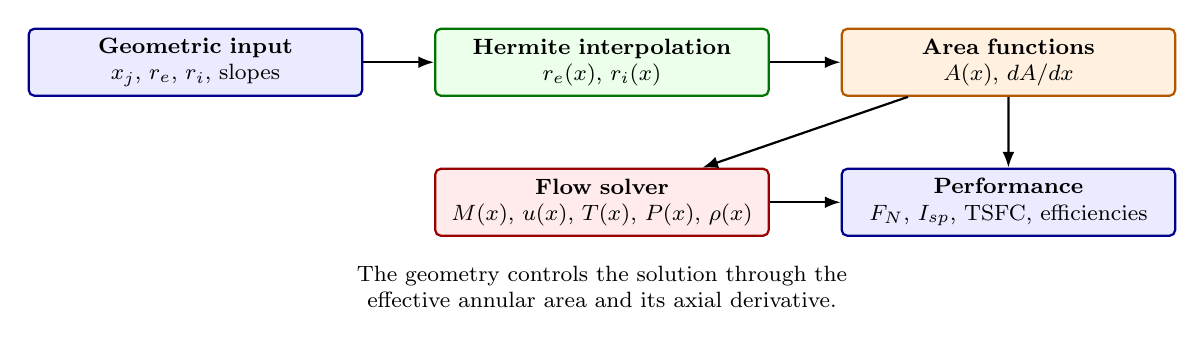
\begin{tikzpicture}[scale=0.95]
    \node[blockblue, text width=4.0cm] (geom) at (0,0) {\textbf{Geometric input}\\$x_j$, $r_e$, $r_i$, slopes};
    \node[blockgreen, text width=4.0cm, right=0.9cm of geom] (hermite) {\textbf{Hermite interpolation}\\$r_e(x)$, $r_i(x)$};
    \node[blockorange, text width=4.0cm, right=0.9cm of hermite] (area) {\textbf{Area functions}\\$A(x)$, $dA/dx$};
    \node[blockred, text width=4.0cm, below=0.9cm of hermite] (flow) {\textbf{Flow solver}\\$M(x)$, $u(x)$, $T(x)$, $P(x)$, $\rho(x)$};
    \node[blockblue, text width=4.0cm, below=0.9cm of area] (perf) {\textbf{Performance}\\$F_N$, $I_{sp}$, TSFC, efficiencies};
    \draw[arrow] (geom) -- (hermite);
    \draw[arrow] (hermite) -- (area);
    \draw[arrow] (area) -- (flow);
    \draw[arrow] (flow) -- (perf);
    \draw[arrow] (area) -- (perf);
    \node[font=\footnotesize, align=center, below=0.25cm of flow, text width=8.5cm] {
    The geometry controls the solution through the effective annular area and its axial derivative.
    };
\end{tikzpicture}%
}
\caption{Conceptual coupling between parametric geometry and the one-dimensional RAMJET flow solver.}
\label{fig:geometry_flow_coupling}
\end{figure}
\subsection{Geometric Continuity and Hermite Interpolation}
A key requirement of the geometric model is to avoid abrupt changes in radius, area, or area derivative. Discontinuities in $A(x)$ or $dA/dx$ may introduce artificial numerical oscillations in the computed Mach number, pressure, temperature, and velocity. For this reason, the external and internal radius functions are required to be continuous and differentiable:
\begin{equation}
r_e(x),\; r_i(x) \in C^1.
\label{eq:c1_condition}
\end{equation}
At each geometric node $x_j$, this condition implies continuity of the radius:
\begin{equation}
r^{(j-1)}(x_j)=r^{(j)}(x_j),
\label{eq:radius_continuity}
\end{equation}
and continuity of the slope:
\begin{equation}
\left.
\frac{dr^{(j-1)}}{dx}
\right|_{x_j}
=
\left.
\frac{dr^{(j)}}{dx}
\right|_{x_j}.
\label{eq:slope_continuity}
\end{equation}
To satisfy these conditions, cubic Hermite interpolation was used to construct the radius profiles. Cubic Hermite interpolation was selected because it allows the radius and slope to be prescribed at each geometric node, providing a smooth $C^1$ representation suitable for numerical differentiation and integration \cite{Burden2011}. For a generic interval
\begin{equation}
x\in[x_j,x_{j+1}],
\qquad
\Delta x_j=x_{j+1}-x_j,
\end{equation}
the local dimensionless coordinate is defined as
\begin{equation}
\xi_j=\frac{x-x_j}{\Delta x_j},
\qquad
0\leq \xi_j \leq 1.
\end{equation}
For a generic radius function $r(x)$, with known endpoint values and slopes,
\begin{equation}
r(x_j)=r_j,\qquad r(x_{j+1})=r_{j+1},
\end{equation}
\begin{equation}
r'(x_j)=m_j,\qquad r'(x_{j+1})=m_{j+1},
\end{equation}
the Hermite polynomial is written as
\begin{equation}
r_j(x)
=
h_{00}(\xi_j)r_j
+
h_{10}(\xi_j)\Delta x_jm_j
+
h_{01}(\xi_j)r_{j+1}
+
h_{11}(\xi_j)\Delta x_jm_{j+1}.
\label{eq:hermite_polynomial}
\end{equation}
The basis functions are
\begin{equation}
h_{00}(\xi)=2\xi^3-3\xi^2+1,
\end{equation}
\begin{equation}
h_{10}(\xi)=\xi^3-2\xi^2+\xi,
\end{equation}
\begin{equation}
h_{01}(\xi)=-2\xi^3+3\xi^2,
\end{equation}
\begin{equation}
h_{11}(\xi)=\xi^3-\xi^2.
\end{equation}
The derivative of the radius function is obtained from
\begin{equation}
\frac{d}{dx}
=
\frac{1}{\Delta x_j}
\frac{d}{d\xi_j}.
\end{equation}
Thus, the derivative of the Hermite polynomial is
\begin{equation}
\frac{dr_j}{dx}
=
\frac{1}{\Delta x_j}
\left[
h'_{00}(\xi_j)r_j
+
h'_{01}(\xi_j)r_{j+1}
\right]
+
h'_{10}(\xi_j)m_j
+
h'_{11}(\xi_j)m_{j+1}.
\label{eq:hermite_derivative}
\end{equation}
This procedure is applied independently to $r_e(x)$ and $r_i(x)$. Once both radius functions and their derivatives are available, the model computes $A(x)$ and $dA/dx$ at any point required by the numerical solver.
\begin{figure}[H]
\centering
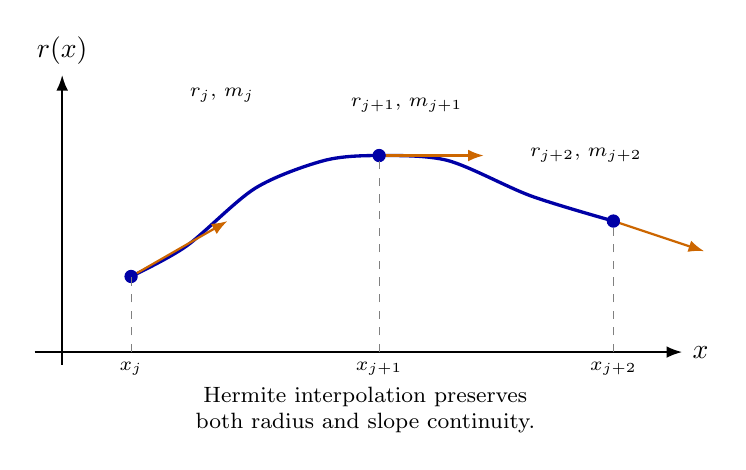
\begin{tikzpicture}[x=3.5cm,y=3.2cm]
    \draw[-{Latex[length=2mm]}, thick] (-0.1,0) -- (2.25,0) node[right] {$x$};
    \draw[-{Latex[length=2mm]}, thick] (0,-0.05) -- (0,1.1) node[above] {$r(x)$};
    \coordinate (P0) at (0.25,0.30);
    \coordinate (P1) at (1.15,0.78);
    \coordinate (P2) at (2.00,0.52);
    \draw[very thick, blue!65!black]
    plot[smooth] coordinates {
        (0.25,0.30) (0.45,0.42) (0.70,0.65) (0.95,0.76)
        (1.15,0.78) (1.40,0.76) (1.70,0.62) (2.00,0.52)
    };
    \draw[orange!80!black, thick, -{Latex[length=2mm]}] (P0) -- ++(0.35,0.22);
    \draw[orange!80!black, thick, -{Latex[length=2mm]}] (P1) -- ++(0.38,0.00);
    \draw[orange!80!black, thick, -{Latex[length=2mm]}] (P2) -- ++(0.33,-0.12);
    \filldraw[blue!65!black] (P0) circle (2.2pt);
    \filldraw[blue!65!black] (P1) circle (2.2pt);
    \filldraw[blue!65!black] (P2) circle (2.2pt);
    \node[font=\scriptsize, below] at (0.25,0) {$x_j$};
    \node[font=\scriptsize, below] at (1.15,0) {$x_{j+1}$};
    \node[font=\scriptsize, below] at (2.00,0) {$x_{j+2}$};
    \draw[dashed, gray] (0.25,0) -- (P0);
    \draw[dashed, gray] (1.15,0) -- (P1);
    \draw[dashed, gray] (2.00,0) -- (P2);
    \node[font=\scriptsize, align=center] at (0.58,1.02) {$r_j$, $m_j$};
    \node[font=\scriptsize, align=center] at (1.25,0.98) {$r_{j+1}$, $m_{j+1}$};
    \node[font=\scriptsize, align=center] at (1.90,0.78) {$r_{j+2}$, $m_{j+2}$};
    \node[font=\footnotesize, align=center, text width=6cm] at (1.10,-0.23) {
    Hermite interpolation preserves both radius and slope continuity.
    };
\end{tikzpicture}
\caption{Cubic Hermite interpolation used to construct smooth radius profiles from geometric nodes, radius values, and prescribed slopes.}
\label{fig:hermite_geometry}
\end{figure}
\subsection{Nodal Discretization of the Computational Domain}
The numerical implementation is based on a nodal discretization of the one-dimensional computational domain. Although the RAMJET is physically organized into inlet, diffuser, combustion chamber, throat, and nozzle regions, the numerical solver evaluates the flow through a finite set of nodes distributed along the axial coordinate. Therefore, the discretization is not defined to describe the engine zones again, but to establish the computational points where the geometric and thermodynamic variables are evaluated.
The engine length is represented by the interval
\begin{equation}
x\in[0,L],
\end{equation}
where $L$ is the total length of the model. This interval is divided into $N$ computational nodes:
\begin{equation}
x_k = k\Delta x,
\qquad
k=0,1,2,\ldots,N,
\label{eq:nodal_grid}
\end{equation}
where $\Delta x$ is the spatial step between two consecutive nodes.
At each node $x_k$, the model evaluates and stores the local geometric variables:
\begin{equation}
A_k,
\qquad
\left(\frac{dA}{dx}\right)_k,
\end{equation}
and the local flow variables:
\begin{equation}
u_k,\;
M_k,\;
T_k,\;
P_k,\;
\rho_k.
\label{eq:nodal_variables}
\end{equation}
The nodal structure allows the model to solve the internal flow as a marching process along the engine. Once the velocity is obtained at a new node, the remaining variables are updated using the thermodynamic relations of the model. In this way, the numerical method provides continuous profiles of Mach number, velocity, temperature, pressure, density, effective area, and area derivative.
\begin{figure}[H]
\centering
\resizebox{1.2\textwidth}{!}{%
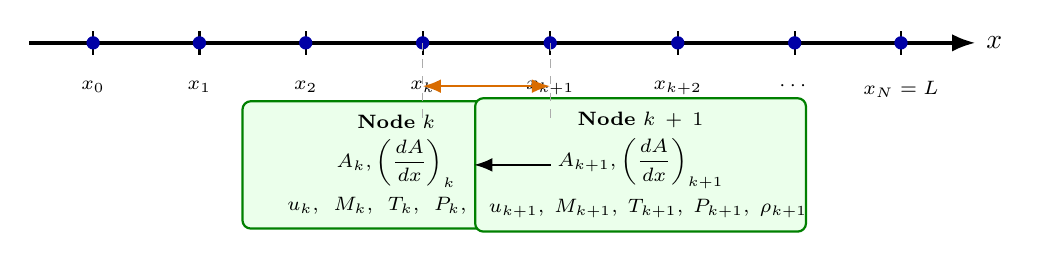
\begin{tikzpicture}[x=1.35cm,y=1cm,>=Latex]
\draw[very thick,->] (0,0) -- (8.9,0) node[right] {$x$};
\foreach \x/\lab in {
    0.6/{$x_0$},
    1.6/{$x_1$},
    2.6/{$x_2$},
    3.7/{$x_k$},
    4.9/{$x_{k+1}$},
    6.1/{$x_{k+2}$},
    7.2/{$\cdots$},
    8.2/{$x_N=L$}
}{
    \draw[thick] (\x,0.15) -- (\x,-0.15);
    \filldraw[blue!65!black] (\x,0) circle (2.2pt);
    \node[font=\scriptsize, below=6pt] at (\x,-0.15) {\lab};
}
\draw[<->, thick, orange!85!black] (3.7,-0.55) -- (4.9,-0.55);
\node[font=\scriptsize, below=2pt] at (4.3,-0.55) {$\Delta x$};
\node[
    draw=green!50!black,
    fill=green!8,
    rounded corners=3pt,
    thick,
    align=center,
    font=\scriptsize,
    text width=3.55cm,
    minimum height=1.15cm,
    inner sep=5pt
] (nodek) at (3.45,-1.55)
{\textbf{Node $k$}\\[1mm]
$A_k,\left(\dfrac{dA}{dx}\right)_k$\\[1mm]
$u_k,\;M_k,\;T_k,\;P_k,\;\rho_k$};
\node[
    draw=green!50!black,
    fill=green!8,
    rounded corners=3pt,
    thick,
    align=center,
    font=\scriptsize,
    text width=3.85cm,
    minimum height=1.15cm,
    inner sep=5pt
] (nodekp) at (5.75,-1.55)
{\textbf{Node $k+1$}\\[1mm]
$A_{k+1},\left(\dfrac{dA}{dx}\right)_{k+1}$\\[1mm]
$u_{k+1},\;M_{k+1},\;T_{k+1},\;P_{k+1},\;\rho_{k+1}$};
\draw[->, thick] (nodek.east) -- (nodekp.west);
\draw[dashed, gray!65] (3.7,0) -- (3.7,-0.95);
\draw[dashed, gray!65] (4.9,0) -- (4.9,-0.95);
\end{tikzpicture}%
}
\caption{Nodal discretization of the one-dimensional computational domain. The solver advances from node $k$ to node $k+1$, updating the local geometry, area derivative, velocity, Mach number, temperature, pressure, and density.}
\label{fig:nodal_discretization}
\end{figure}
\subsection{Numerical Solution Procedure}
The numerical solution was implemented in MATLAB using a sequential procedure. The model first defines the operating conditions, geometric parameters, thermodynamic properties, and fuel parameters. Then, the geometry module constructs the functions $r_e(x)$ and $r_i(x)$, from which $A(x)$ and $dA/dx$ are obtained. These functions are then supplied to the flow solver.
The most sensitive part of the numerical method is the integration of the area--velocity equation:
\begin{equation}
\frac{du}{dx}
=
f(x,u)
=
\frac{u}{M^2-1}
\frac{1}{A}
\frac{dA}{dx}.
\label{eq:numerical_velocity}
\end{equation}
This equation is integrated in the adiabatic regions of the engine using an adaptive Runge--Kutta method. In MATLAB, this was implemented using the solver \texttt{ode45}, which is based on an explicit Runge--Kutta pair with automatic step-size control. This type of adaptive integration is suitable for ordinary differential equations where the solution may change rapidly due to geometric gradients or near-critical flow conditions \cite{Burden2011}. Conceptually, the integration can be expressed as
\begin{equation}
[x,u]
=
\texttt{ode45}
\left(
f(x,u),[x_{ini},x_{fin}],u_{ini}
\right).
\label{eq:ode45}
\end{equation}
The use of an adaptive solver is important because the derivative $du/dx$ can change rapidly when the area gradient varies or when the flow approaches the sonic condition. In particular, the denominator $M^2-1$ makes the numerical solution sensitive near $M=1$. Therefore, the solver must control the integration step to avoid artificial divergence or non-physical oscillations.
After the velocity is obtained at a new computational point, the thermodynamic variables are updated in a fixed sequence. For an adiabatic region with total temperature $T_{0,j}$, the static temperature is computed as
\begin{equation}
T_{k+1}
=
T_{0,j}
-
\frac{u_{k+1}^{2}}{2c_p}.
\label{eq:temperature_update}
\end{equation}
The local speed of sound is
\begin{equation}
c_{k+1}
=
\sqrt{\gamma R T_{k+1}},
\end{equation}
and the Mach number is updated as
\begin{equation}
M_{k+1}
=
\frac{u_{k+1}}{c_{k+1}}.
\end{equation}
The density is obtained from the conservation of mass:
\begin{equation}
\rho_{k+1}
=
\frac{\dot{m}}
{u_{k+1}A_{k+1}},
\label{eq:density_update}
\end{equation}
and the pressure is calculated using the ideal gas equation:
\begin{equation}
P_{k+1}
=
\rho_{k+1}RT_{k+1}.
\label{eq:pressure_update}
\end{equation}
The numerical update sequence is therefore
\begin{equation}
A_{k+1},\left(\frac{dA}{dx}\right)_{k+1}
\rightarrow
u_{k+1}
\rightarrow
T_{k+1}
\rightarrow
c_{k+1}
\rightarrow
M_{k+1}
\rightarrow
\rho_{k+1}
\rightarrow
P_{k+1}.
\label{eq:update_sequence}
\end{equation}
This procedure is repeated through the computational domain, while applying the corresponding physical model in each region: aerodynamic compression before combustion, heat addition and pressure loss in the combustion chamber, sonic condition at the throat, and supersonic expansion in the divergent nozzle.
% =========================================================================
\section{Results and Discussion}
\label{sec:results}
% =========================================================================
The numerical model was evaluated using a baseline supersonic operating condition in order to verify the physical consistency of the RAMJET simulation. The analysis focuses on the axial evolution of the main flow variables, the thermodynamic state at the characteristic stations of the engine, the global performance metrics, and the sensitivity of the model to selected operating and geometric parameters. In this section, the results are interpreted not only as numerical outputs, but also as evidence of the physical coherence of the proposed parametrizable model.
\subsection{Baseline Simulation Parameters}
The baseline case corresponds to a supersonic flight condition with a free-stream Mach number of $M_\infty=2.0$. The atmospheric conditions were defined by a static temperature of $T_\infty=223.15$ K and a static pressure of $P_\infty=26.5$ kPa. Jet-A1 was considered as the reference fuel. The selected condition was used as the reference point for verifying the expected operating sequence of the RAMJET engine: inlet compression, heat addition, sonic throat condition, supersonic expansion, and thrust generation.
\begin{table}[H]
\centering
\caption{Baseline design and operating parameters.}
\label{tab:baseline_parameters}
\begin{tabular}{llll}
\toprule
\textbf{Group} & \textbf{Parameter} & \textbf{Symbol} & \textbf{Value} \\
\midrule
Operation & Flight Mach number & $M_\infty$ & 2.00 \\
Operation & Static flight temperature & $T_\infty$ & 223.15 K \\
Operation & Static flight pressure & $P_\infty$ & 26.5 kPa \\
Inlet & Post-inlet design Mach number & $M_{2,design}$ & 0.18 \\
Inlet & Total pressure recovery & $\eta_d$ & 0.92 \\
Combustion & Fuel-to-air ratio & $f$ & 0.03 \\
Combustion & Combustion efficiency & $\eta_b$ & 0.98 \\
Combustion & Combustor total pressure ratio & $\sigma_b$ & 0.98 \\
Geometry & Inlet diameter & $D_{inlet}$ & 192 mm \\
Geometry & Chamber diameter & $D_c$ & 180 mm \\
Geometry & Compatible throat diameter & $D_5$ & 139.7 mm \\
Geometry & Exit diameter & $D_6$ & 184 mm \\
\bottomrule
\end{tabular}
\end{table}
\subsection{Effective Area and Area Gradient}
The parametrized geometry generated by the MATLAB model defines the external duct radius $r_e(x)$, the internal spike radius $r_i(x)$, and the resulting annular flow passage. This geometric construction is the main input of the aerodynamic model, since the effective area $A(x)$ and its axial derivative $dA/dx$ directly determine the acceleration or deceleration of the compressible flow through the area--velocity equation.
\begin{figure}[H]
\centering
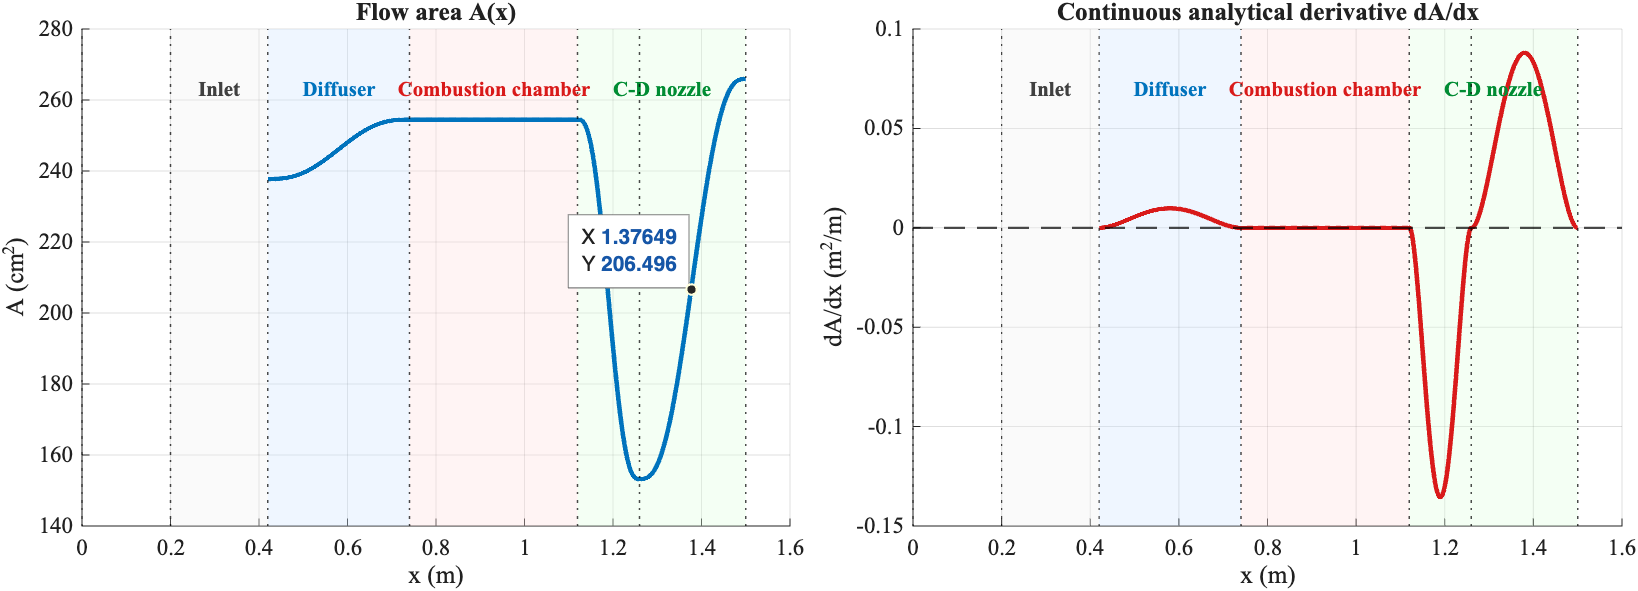
\includegraphics[width=1.2\textwidth]{dx.png}
\caption{Effective area $A(x)$ and axial derivative $dA/dx$ obtained from the parametrized RAMJET geometry generated in MATLAB. The smooth derivative reduces artificial numerical oscillations in Mach number, pressure, and temperature.}
\label{fig:area_derivative}
\end{figure}
The smooth behavior of $dA/dx$ is an important aspect of the numerical solution. Since the velocity differential equation depends explicitly on the area derivative, abrupt discontinuities in $dA/dx$ may generate non-physical oscillations in the computed velocity, Mach number, pressure, or temperature. The results shown in Figure~\ref{fig:area_derivative} confirm that the Hermite-based parametrization produces a continuous area distribution and a smooth derivative, which is necessary for stable integration of the area--velocity equation.
This result is relevant because it validates one of the central assumptions of the computational model: the geometry can be modified parametrically without breaking the numerical consistency of the solver. In other words, the geometry is not only visually continuous, but also mathematically suitable for being used as an input to the differential flow model.
\subsection{Axial Thermodynamic Behavior}
The computed axial profiles reproduce the main physical behavior expected in a RAMJET engine. At the inlet and diffuser, the flow is decelerated from supersonic to subsonic conditions. This deceleration produces an increase in static pressure and static temperature, which represents the aerodynamic compression process required before combustion.
Inside the combustion chamber, the temperature increases significantly due to the heat released by the injected fuel. The pressure decreases slightly as a consequence of the pressure loss factor introduced in the combustor model. At the nozzle throat, the flow reaches the sonic condition, $M_5=1$. Downstream of the throat, the divergent nozzle expands the hot gases and accelerates the flow toward the exit.
\begin{figure}[H]
\centering
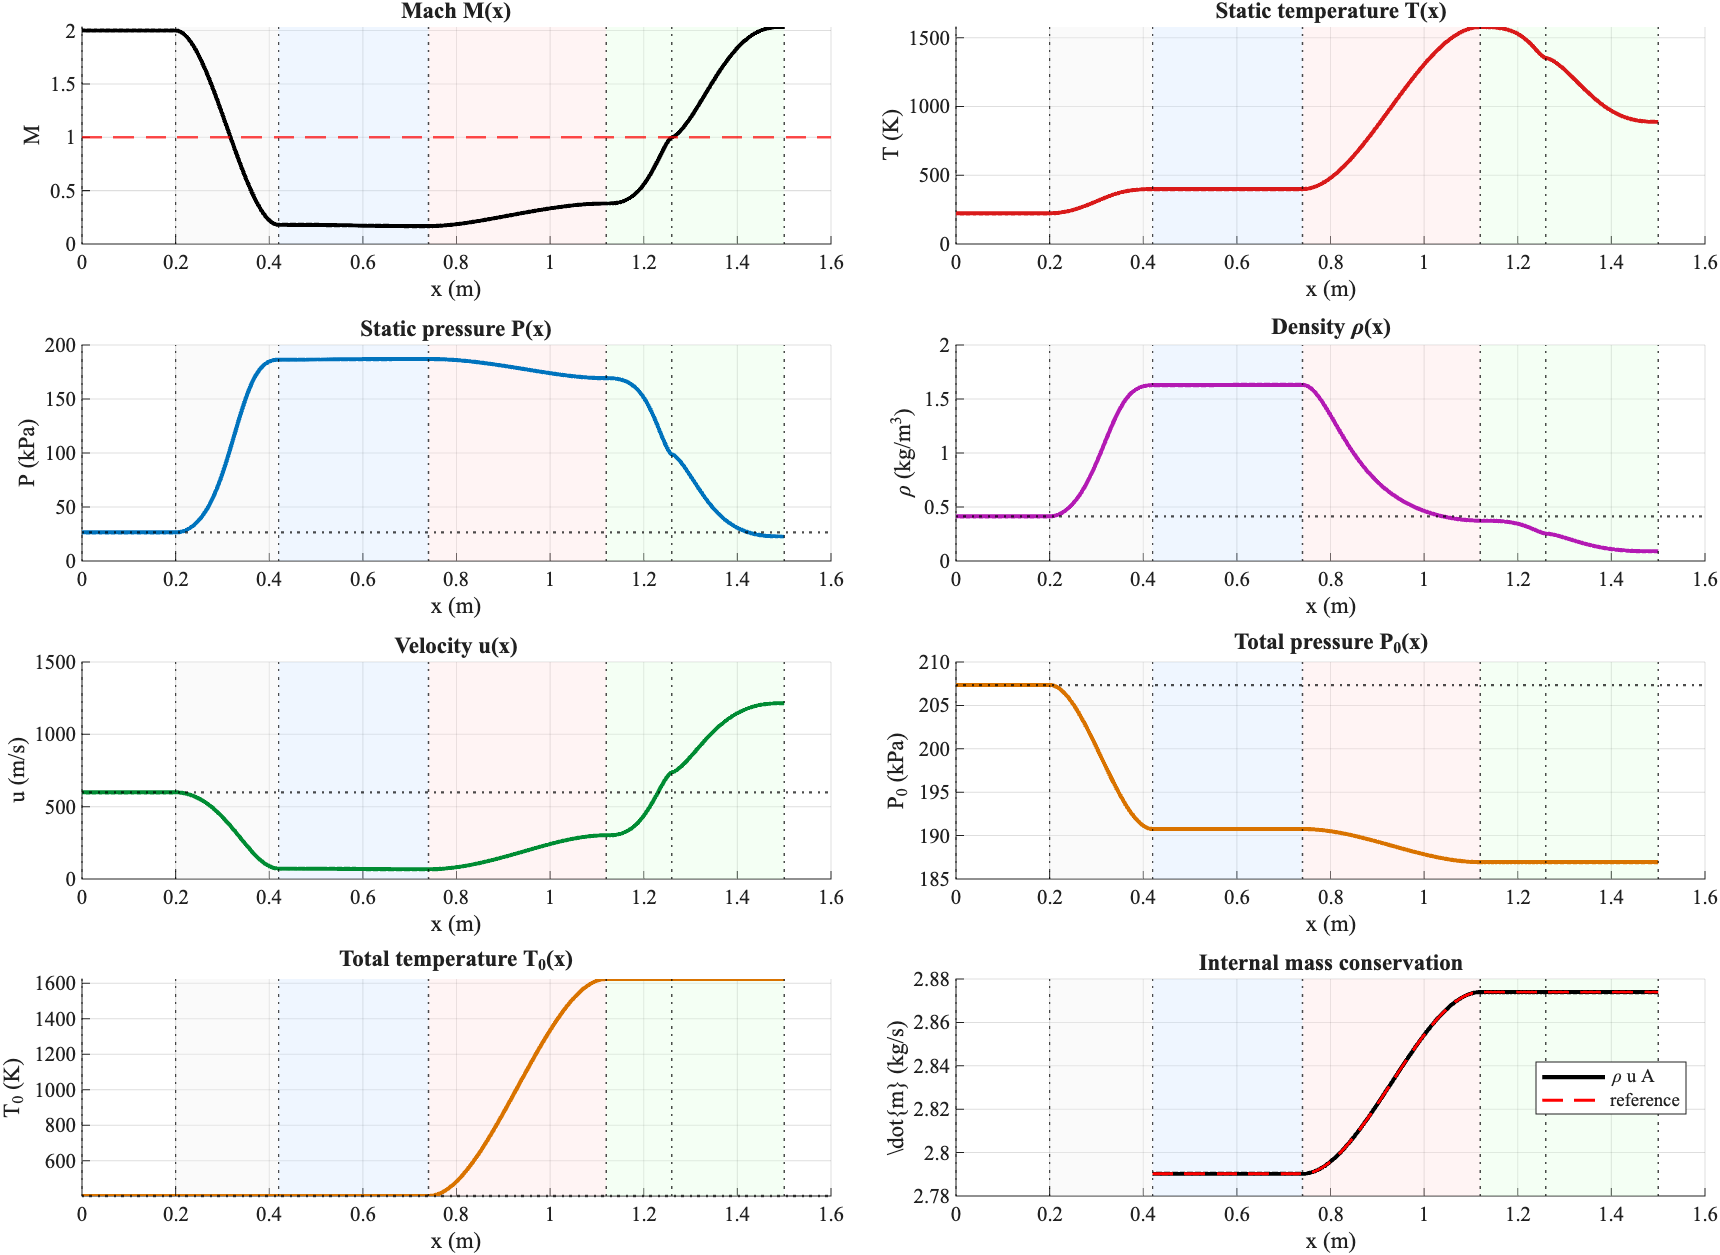
\includegraphics[width=1.2\textwidth]{RAMJET Thermodynamic Parameters by Zone.png}
\caption{Axial thermodynamic and aerodynamic profiles obtained from the MATLAB RAMJET simulator for the baseline case. The curves show the compression process, heat addition in the combustor, sonic throat condition, and supersonic nozzle expansion.}
\label{fig:thermodynamic_profiles}
\end{figure}
Figure~\ref{fig:thermodynamic_profiles} shows that the Mach number is the key variable controlling the interpretation of the flow in each region. Before combustion, the model reduces the Mach number to allow a physically consistent heat-addition process. In the nozzle throat, the imposed sonic condition defines the critical section of the engine. Finally, the divergent nozzle increases the Mach number again, producing a supersonic exit flow. This behavior confirms that the model does not simply calculate isolated thermodynamic states, but reproduces the sequence required for RAMJET operation.
\subsection{Flow Properties at Characteristic Stations}
\begin{table}[H]
\centering
\caption{Thermodynamic variables at the main engine stations for the baseline case.}
\label{tab:station_properties}
\begin{tabular}{llllllll}
\toprule
\textbf{Station} & \textbf{Zone} & $\mathbf{M}$ & $\mathbf{T}$ \textbf{(K)} & $\mathbf{P}$ \textbf{(kPa)} & $\boldsymbol{\rho}$ \textbf{(kg/m$^3$)} & $\mathbf{u}$ \textbf{(m/s)} & $\mathbf{T_0}$ \textbf{(K)} \\
\midrule
$x_0$ & Free stream & 2.000 & 223.2 & 26.5 & 0.414 & 598.9 & 401.7 \\
$x_2$ & Post-inlet & 0.180 & 399.1 & 186.5 & 1.628 & 72.1 & 401.7 \\
$x_3$ & Chamber inlet & 0.168 & 399.4 & 187.0 & 1.631 & 67.2 & 401.7 \\
$x_4$ & Chamber outlet & 0.380 & 1577.9 & 169.3 & 0.374 & 302.2 & 1623.3 \\
$x_5$ & Throat & 1.000 & 1352.8 & 98.8 & 0.254 & 737.3 & 1623.3 \\
$x_6$ & Exit & 2.033 & 888.7 & 22.7 & 0.089 & 1215.0 & 1623.3 \\
\bottomrule
\end{tabular}
\end{table}
Between $x_0$ and $x_2$, the Mach number decreases from $M=2.0$ to $M=0.18$, while the static pressure increases from 26.5 kPa to 186.5 kPa. This result confirms that the inlet and diffuser produce aerodynamic compression before the combustion process. The increase in static pressure is not produced by mechanical work, but by the conversion of kinetic energy into pressure through the geometry of the inlet and diffuser.
Between $x_3$ and $x_4$, the static temperature increases from 399.4 K to 1577.9 K as a result of heat addition in the combustion chamber. At the throat, the model imposes the sonic condition, and in the divergent nozzle the flow accelerates up to $M_6=2.033$, with an exit velocity of $u_6=1215.0$ m/s. This final acceleration is the mechanism that allows the engine to convert the thermal energy released in combustion into kinetic energy and useful thrust.
\subsection{Global Performance Metrics}
\begin{table}[H]
\centering
\caption{Global performance metrics for the baseline case.}
\label{tab:performance_metrics}
\begin{tabular}{lll}
\toprule
\textbf{Metric} & \textbf{Symbol} & \textbf{Value} \\
\midrule
Gross thrust & $F_{gross}$ & 3390.6 N \\
Net thrust & $F_N$ & 1719.4 N \\
Specific impulse & $I_{sp}$ & 2094.6 s \\
Air mass flow rate & $\dot{m}_a$ & 2.790 kg/s \\
Fuel mass flow rate & $\dot{m}_f$ & 0.0837 kg/s \\
Propulsive efficiency & $\eta_{prop}$ & 66.0\% \\
Thermal efficiency & $\eta_{term}$ & 45.9\% \\
Global efficiency & $\eta_{global}$ & 30.3\% \\
Exit Mach number & $M_6$ & 2.033 \\
Mass conservation error & -- & $<10^{-8}$ kg/s \\
\bottomrule
\end{tabular}
\end{table}
The net thrust obtained for the baseline case was $F_N=1719.4$ N. This value is one of the most important indicators of the model because it shows that the complete RAMJET cycle produces useful propulsion after subtracting the incoming momentum of the captured air. In other words, the engine does not only accelerate the exhaust gases internally; it produces a positive momentum balance with respect to the flight condition. This confirms that the selected geometry, combustion parameters, and nozzle expansion are mutually compatible under the baseline operating point.
The difference between gross thrust and net thrust is also relevant. The gross thrust represents the momentum generated at the nozzle exit, whereas the net thrust accounts for the momentum already carried by the incoming air. Since a RAMJET operates at high flight speed, the incoming momentum term is significant. Therefore, the net thrust is the physically meaningful metric for evaluating whether the engine configuration can generate useful propulsive force.
The specific impulse of $I_{sp}=2094.6$ s indicates the relation between the generated thrust and the fuel mass flow rate. This value suggests that, within the simplified assumptions of the one-dimensional model, the baseline configuration uses the injected fuel effectively to produce thrust. However, this result must be interpreted as a preliminary performance estimate, since detailed combustion losses, viscous effects, and shock losses were not explicitly resolved.
The mass conservation error lower than $10^{-8}$ kg/s is another important result. This value indicates that the numerical implementation preserves mass-flow compatibility through the inlet, combustion chamber, throat, and nozzle. Since the model updates density from the continuity relation and uses the effective area provided by the parametrized geometry, a small mass conservation error confirms that the nodal solution is internally consistent. This is particularly important because a RAMJET model can produce misleading thrust values if the mass flow is not conserved accurately across the computational domain.
Finally, the global efficiency of $30.3\%$ results from the combination of the thermal and propulsive efficiencies. The thermal efficiency reflects the conversion of fuel chemical energy into useful gas energy, while the propulsive efficiency measures how effectively this energy is converted into useful momentum change. The obtained value is consistent with the preliminary nature of the model and provides a reference point for future geometric optimization.
\subsection{Trend Validation Against a Reference Model}
The model was compared against the general trends reported in a previous RAMJET reference study developed by Dallos Trujillo and Bayona Roa \cite{Dallos2024}. This comparison was not intended as a point-to-point validation because the geometry, inlet assumptions, simulation conditions, and detailed formulation of both models are not identical. Instead, the objective was to verify whether the proposed parametrized model reproduces the expected physical tendencies of a generic RAMJET engine.
The validation matrix considered flight Mach numbers in the range
\begin{equation}
M_\infty \in [2.3,4.0],
\end{equation}
and four fuels: methane, Jet-A1, hydrogen, and octane. The analysis showed that the thrust-specific fuel consumption decreases as the flight Mach number increases. This trend is physically consistent because higher flight speeds increase the dynamic compression of the incoming flow, reducing the relative amount of additional fuel energy required to reach the target combustion condition.
\subsection{Sensitivity Analysis and Geometric Parametrization Validation}
A sensitivity analysis was performed by varying one parameter at a time while maintaining the remaining variables at their baseline values. The objective was not only to determine which variables most strongly affect net thrust, but also to verify that the parametrized geometry produces physically meaningful changes in the numerical solution.
\begin{table}[H]
\centering
\caption{Summary of the sensitivity analysis.}
\label{tab:sensitivity_summary}
\begin{tabular}{llll}
\toprule
\textbf{Parameter} & \textbf{Range} & \textbf{Net thrust range (N)} & $\boldsymbol{\Delta F_N}$ \textbf{(\%)} \\
\midrule
$M_\infty$ & 1.6--3.0 & 858--6656 & +287 \\
$M_{2,design}$ & 0.15--0.30 & 1411--2599 & +51 \\
$r_{inlet}$ & 86.4--105.6 mm & 1269--2148 & +69 \\
$f$ & 0.020--0.045 & 1220--2340 & +36 \\
$\eta_d$ & 0.86--0.98 & 1561--1878 & +18 \\
$r_{i,peak}$ & 52.2--63.8 mm & 1638--1792 & +9 \\
$r_{e,exit}$ & 82.8--101.2 mm & 1678--1723 & +3 \\
$\sigma_b$ & 0.94--1.00 & 1694--1732 & +2 \\
$r_c$ & 81.0--99.0 mm & $\Delta F_N<0.001$ N & $\approx 0$ \\
\bottomrule
\end{tabular}
\end{table}
The strongest sensitivity was obtained for the flight Mach number. Increasing $M_\infty$ produces a significant increase in net thrust because the kinetic energy and dynamic compression of the incoming flow increase. This confirms the expected behavior of a RAMJET engine: the system becomes more effective as the incoming flow provides more kinetic energy for aerodynamic compression.
The inlet radius was the most influential geometric parameter. This result is physically consistent because $r_{inlet}$ modifies the capture area and, therefore, the air mass flow rate entering the engine. A larger inlet radius increases the available air for combustion and expansion, which increases thrust. This behavior validates the geometric parametrization because a change in the inlet radius is correctly reflected in the area distribution, mass flow rate, and final propulsion output.
The post-inlet design Mach number also produced a strong effect. This variable controls the thermodynamic state entering the combustion chamber. A higher $M_{2,design}$ preserves more kinetic energy after the inlet, while a lower value produces stronger deceleration and higher static pressure recovery. Therefore, this parameter represents a trade-off between compression, combustion compatibility, and nozzle expansion.
The fuel-to-air ratio directly affects the amount of heat added in the combustion chamber. Increasing $f$ raises the gas temperature and increases the energy available for expansion, producing higher thrust. However, this also increases fuel consumption, which means that higher thrust does not necessarily imply better overall performance.
The parameters $r_{i,peak}$ and $r_{e,exit}$ showed lower influence than $r_{inlet}$ in the evaluated range. This does not mean that the spike and nozzle exit are unimportant; rather, it indicates that isolated variations of these parameters produce smaller changes under the selected baseline condition. The result suggests that future optimization should vary the inlet, spike, throat, and nozzle geometry simultaneously, instead of modifying each parameter independently. This behavior is consistent with RAMJET propulsion theory, where the incoming Mach number, inlet capture area, pressure recovery, and heat addition strongly affect the momentum balance and the final net thrust \cite{Hill1992,Mattingly2006,Heiser1994}.
To support the sensitivity analysis, the most representative MATLAB results are included in Figures~\ref{fig:sensitivity_mach}--\ref{fig:sensitivity_m2design}. These figures correspond to the simulations where the most influential operating and geometric parameters were varied.
\begin{figure}[H]
\centering
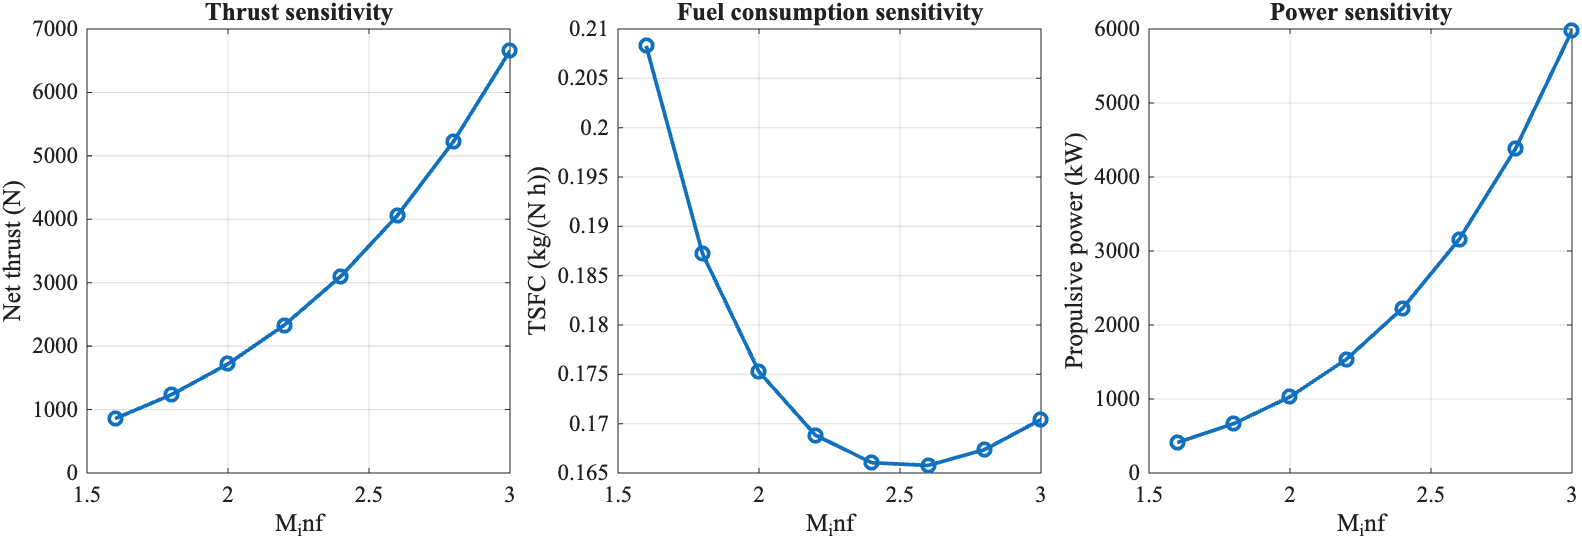
\includegraphics[width=0.90\textwidth]{Sensitivity - Flight Mach number.png}
\caption{Sensitivity of net thrust to flight Mach number. This result shows the dominant influence of the incoming supersonic flow condition on RAMJET performance.}
\label{fig:sensitivity_mach}
\end{figure}
\begin{figure}[H]
\centering
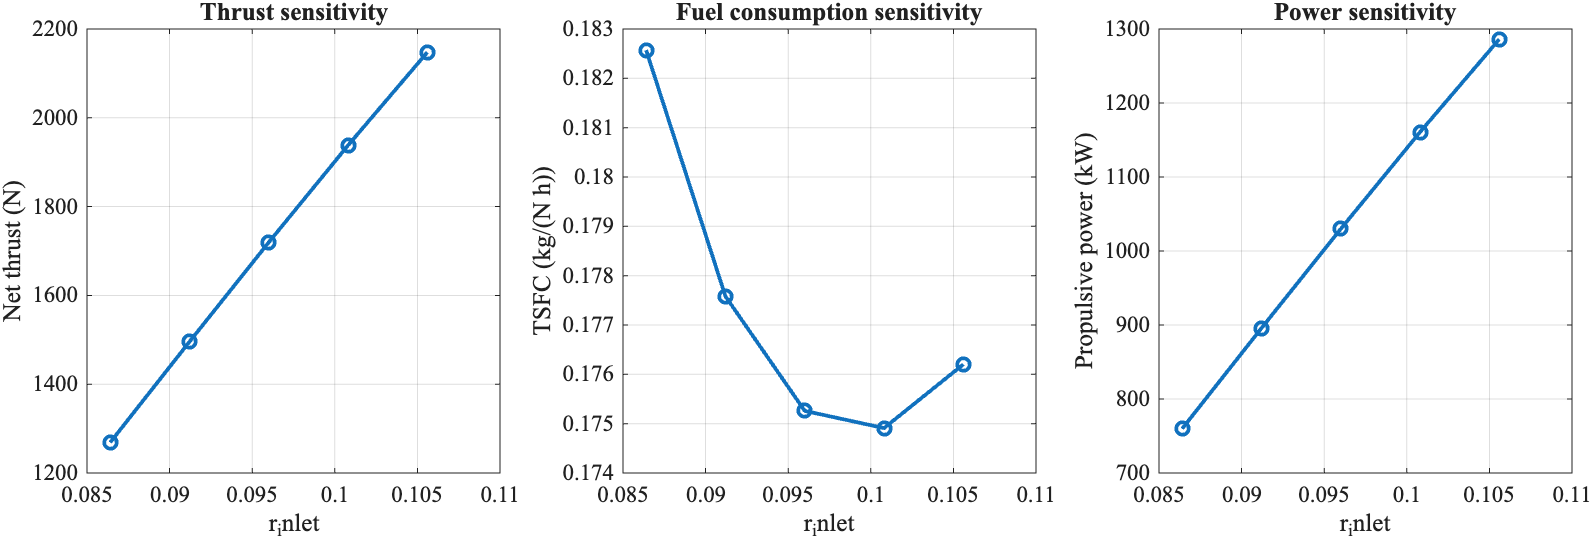
\includegraphics[width=0.90\textwidth]{Sensitivity - Inlet radius.png}
\caption{Sensitivity of net thrust to inlet radius. The variation of $r_{inlet}$ modifies the capture area and validates the influence of the parametrized geometry on the mass flow rate and thrust.}
\label{fig:sensitivity_inlet_radius}
\end{figure}
\begin{figure}[H]
\centering
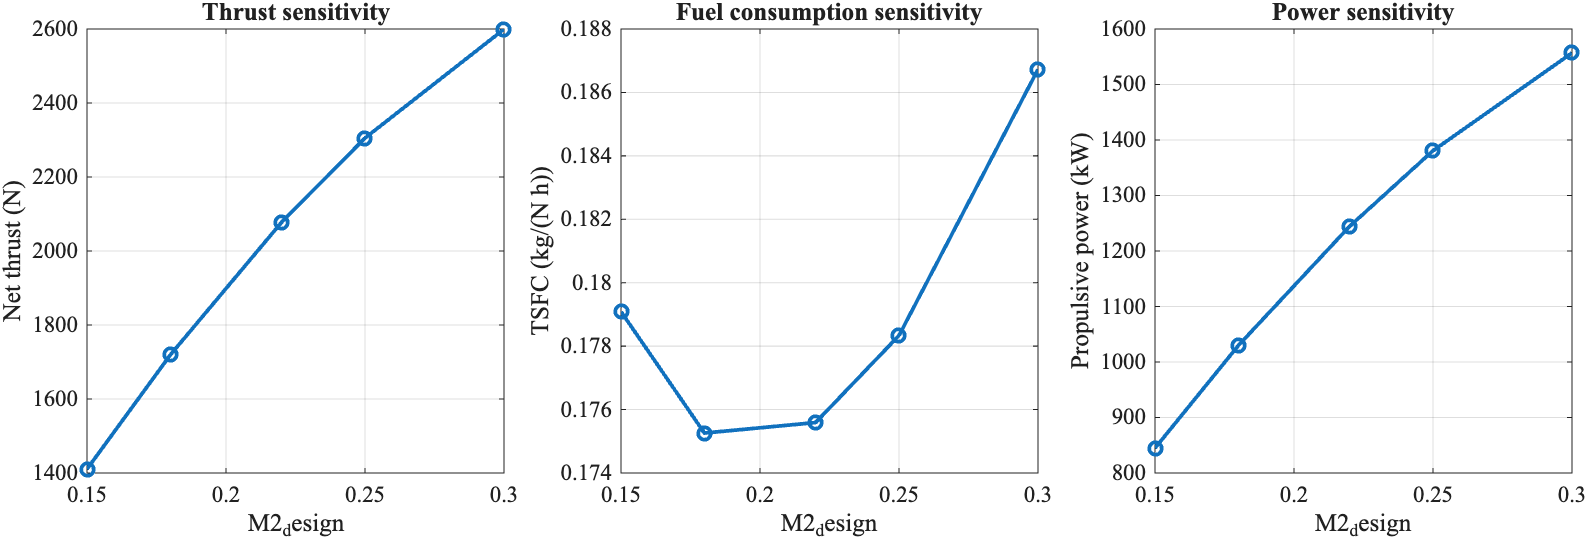
\includegraphics[width=0.90\textwidth]{Sensitivity - Post-inlet Mach.png}
\caption{Sensitivity of net thrust to the post-inlet design Mach number. This parameter affects the balance between aerodynamic compression, combustion compatibility, and nozzle expansion.}
\label{fig:sensitivity_m2design}
\end{figure}
The combined sensitivity results confirm that the parametrized geometry is not a merely graphical feature of the model. On the contrary, geometric variations modify the effective area function, the mass flow rate, the area--velocity coupling, and the final performance metrics. Therefore, the sensitivity analysis provides a numerical validation of the geometric parametrization approach used in the RAMJET model.
% =========================================================================
\section{Conclusions, Limitations, and Future Work}
\label{sec:conclusions}
% =========================================================================
\subsection{Conclusions}
In this work, a one-dimensional numerical model of a supersonic RAMJET engine with parametrizable geometry was developed and implemented in MATLAB. The model integrates the geometric definition of the engine, compressible-flow relations, the area--velocity equation, the combustion energy balance, the convergent-divergent nozzle expansion, and the calculation of global performance metrics. This formulation makes it possible to evaluate the thermodynamic and aerodynamic evolution of the flow from the inlet to the nozzle exit.
The proposed model successfully reproduced the expected physical sequence of a RAMJET engine. In the inlet and diffuser regions, the incoming supersonic flow was decelerated and compressed. In the combustion chamber, heat addition produced a significant increase in gas temperature. At the nozzle throat, the sonic condition was imposed, and in the divergent section the gases were accelerated toward supersonic exit conditions. The baseline case generated positive net thrust, confirming the physical consistency of the model within the assumptions adopted.
One of the main contributions of this work is the use of a parametrizable geometric representation based on the external duct radius $r_e(x)$ and the internal spike radius $r_i(x)$. From these functions, the effective annular area $A(x)$ and its spatial derivative $dA/dx$ were obtained and directly coupled with the flow solution. This approach allows the inlet, spike, combustion chamber, throat, and nozzle geometry to be modified without reconstructing the entire computational model.
The implementation of cubic Hermite interpolation allowed smooth radius profiles to be generated while preserving geometric continuity. This was important because the area derivative appears explicitly in the area--velocity equation. Therefore, avoiding abrupt discontinuities in $A(x)$ and $dA/dx$ improved the numerical stability of the model and reduced the possibility of non-physical oscillations in the computed flow variables.
The baseline simulation showed a coherent RAMJET behavior, with aerodynamic compression before combustion, temperature rise inside the chamber, sonic condition at the throat, expansion through the divergent nozzle, and supersonic exit flow. The model produced a net thrust of $1719.4$ N, a specific impulse of $2094.6$ s, an exit Mach number of $2.033$, and a global efficiency of $30.3\%$ for the selected operating condition.
The sensitivity analysis showed that the most influential variables on the net thrust were the flight Mach number, the post-inlet design Mach number, and the inlet radius. These parameters directly affect the kinetic energy of the incoming flow and the captured air mass flow rate. The fuel-to-air ratio also had a relevant effect because it controls the amount of thermal energy added in the combustion chamber. In contrast, isolated variations in local geometric parameters, such as the chamber radius or combustor pressure ratio, produced smaller changes in the baseline model.
Overall, the developed model constitutes a reproducible computational methodology for preliminary RAMJET analysis. Its main strength is the direct connection between parametrized geometry and flow evolution, allowing different configurations to be evaluated with reduced computational cost. Therefore, the model can be used as a basis for future sensitivity studies, conceptual design exploration, and preliminary geometric optimization of supersonic air-breathing propulsion systems.
\subsection{Limitations}
The model developed in this work is subject to several limitations derived from its simplified formulation. First, the flow is modeled as one-dimensional and steady. Therefore, three-dimensional effects, transient phenomena, viscous boundary layers, turbulence, flow separation, secondary flows, and non-uniform profiles across the engine section are not explicitly resolved.
Second, the inlet compression process is represented using a global aerodynamic compression approach and pressure recovery factor. The model does not explicitly solve the system of oblique and normal shock waves that may appear in the spike, inlet, and diffuser of a real RAMJET engine. Consequently, shock-induced losses and detailed shock-position effects are not directly predicted.
Third, combustion is represented through a simplified energy balance. The model does not include detailed chemical kinetics, finite-rate reactions, turbulent mixing, fuel atomization, flame stabilization, species formation, or pollutant emissions. For this reason, the combustion chamber results should be interpreted as a thermodynamic approximation rather than a detailed combustion simulation.
Fourth, heat transfer through the engine walls is neglected. Although high temperatures are obtained in the combustion chamber and nozzle, the model does not evaluate wall cooling, thermal stresses, material resistance, or structural integrity. Therefore, the results cannot be used directly as a final constructive design criterion.
Fifth, the validation performed in this work is based on physical consistency, conservation of mass, trend comparison, and sensitivity analysis. Due to the limited availability of experimental RAMJET data and real engine geometries, a direct point-to-point experimental validation was not performed. Thus, the model should be considered a preliminary computational tool rather than a fully validated predictive model for a specific real engine.
\subsection{Future Work}
Future developments should incorporate a more detailed supersonic inlet model, including oblique and normal shock relations. This would allow the pressure recovery, Mach number reduction, and shock-induced losses to be predicted with greater physical fidelity.
The combustion chamber model should also be extended to include more detailed combustion physics. Possible improvements include fuel-air mixing models, simplified chemical kinetics, finite-rate heat release, species tracking, and estimation of emissions such as nitrogen oxides. These additions would allow the model to evaluate not only propulsion performance, but also combustion quality and environmental impact.
From a numerical perspective, future work should include a systematic analysis of solver sensitivity, spatial resolution, integration tolerances, and numerical stability near the sonic condition. This would make it possible to quantify how numerical parameters influence the predicted Mach number, pressure, temperature, thrust, and efficiency.
The geometric model could also be expanded by coupling all major geometric variables during optimization. Instead of varying one parameter at a time, future studies should modify the inlet, spike, combustion chamber, throat, and nozzle simultaneously using an optimization algorithm. This would allow the model to search for geometries that maximize thrust, reduce fuel consumption, or improve global efficiency under prescribed flight conditions.
Finally, the model should be compared against experimental measurements, published RAMJET data, or higher-fidelity CFD simulations. Such validation would allow the pressure loss factors, combustion assumptions, and nozzle expansion model to be adjusted, increasing the reliability of the tool for preliminary design applications.
% =========================================================================
% MDPI mandatory sections
% =========================================================================
\authorcontributions{
Conceptualization, S.C.F. and C.B.R.; methodology, S.C.F. and C.B.R.; mathematical formulation, S.C.F.; software implementation, S.C.F.; validation and sensitivity analysis, S.C.F.; formal analysis, S.C.F.; investigation, S.C.F.; writing--original draft preparation, S.C.F.; writing--review and editing, S.C.F. and C.B.R.; supervision, C.B.R. All authors have read and agreed to the final version of the manuscript.
}
\funding{
This research received no external funding.
}
\acknowledgments{
The author gratefully acknowledges the guidance and academic support provided by Camilo Bayona Roa during the development of the undergraduate thesis project. The author also acknowledges the Faculty of Engineering at Pontificia Universidad Javeriana for providing the academic framework in which this research was developed.
}
\conflictsofinterest{
The authors declare no conflict of interest.
}
\abbreviations{
The following nomenclature is used in this manuscript:
\noindent
\begin{tabular}{@{}lllll}
\multicolumn{2}{l}{\textbf{Nomenclature}} &  & \multicolumn{2}{l}{\textbf{Greek letters}} \\
$A$ & Effective flow area &  & $\gamma$ & Specific heat ratio \\
$c$ & Speed of sound &  & $\eta_b$ & Combustion efficiency \\
$c_p$ & Specific heat at constant pressure &  & $\eta_d$ & Inlet pressure recovery \\
$F_N$ & Net thrust &  & $\eta_{prop}$ & Propulsive efficiency \\
$f$ & Fuel-to-air ratio &  & $\eta_{term}$ & Thermal efficiency \\
$g_0$ & Standard gravity &  & $\rho$ & Density \\
$I_{sp}$ & Specific impulse &  & $\sigma_b$ & Combustor pressure ratio \\
$LHV$ & Lower heating value &  &  &  \\
$M$ & Mach number &  & \multicolumn{2}{l}{\textbf{Subscripts}} \\
$\dot{m}$ & Mass flow rate &  & $a$ & Air or free stream \\
$P$ & Static pressure &  & $f$ & Fuel \\
$P_0$ & Total pressure &  & $g$ & Combustion gas \\
$R$ & Gas constant &  & $0$ & Total condition \\
$T$ & Static temperature &  & $2$ & Post-inlet station \\
$T_0$ & Total temperature &  & $4$ & Combustor outlet \\
$u$ & Axial velocity &  & $5$ & Nozzle throat \\
$x$ & Axial coordinate &  & $6$ & Nozzle exit \\
\end{tabular}
}
\reftitle{References}
\begin{thebibliography}{99}
\bibitem{Hill1992}
Hill, P.; Peterson, C. \textit{Mechanics and Thermodynamics of Propulsion}; Addison-Wesley: Reading, MA, USA, 1992.
\bibitem{Mattingly2006}
Mattingly, J.D. \textit{Elements of Propulsion: Gas Turbines and Rockets}; AIAA Education Series: Reston, VA, USA, 2006.
\bibitem{NASA2015}
NASA Glenn Research Center. Ramjet Propulsion. Available online: \url{https://www.grc.nasa.gov/www/k-12/airplane/ramjet.html}.
\bibitem{Anderson2017}
Anderson, J.D. \textit{Introduction to Flight}; McGraw-Hill Education: New York, NY, USA, 2017.
\bibitem{Anderson1990}
Anderson, J.D. \textit{Modern Compressible Flow with Historical Perspective}, 3rd ed.; McGraw-Hill: New York, NY, USA, 1990.
\bibitem{Heiser1994}
Heiser, W.H.; Pratt, D.T. \textit{Hypersonic Airbreathing Propulsion}; American Institute of Aeronautics and Astronautics: Washington, DC, USA, 1994.
\bibitem{Matsuo2005}
Matsuo, K.; Setoguchi, T.; Kudo, K. Shock Waves and Compression Systems in Supersonic Air Intakes. \textit{Progress in Aerospace Sciences} \textbf{2005}, \textit{41}, 471--521.
\bibitem{Burden2011}
Burden, R.L.; Faires, J.D. \textit{Numerical Analysis}, 9th ed.; Brooks/Cole: Boston, MA, USA, 2011.
\bibitem{Bayona2019}
Bayona-Roa, C.; Solís-Chaves, J.S.; Bonilla, J.; Rodriguez-Melendez, A.G.; Castellanos, D. Computational Simulation of PT6A Gas Turbine Engine Operating with Different Blends of Biodiesel---A Transient-Response Analysis. \textit{Energies} \textbf{2019}, \textit{12}, 4258.
\bibitem{Dallos2024}
Dallos Trujillo, A.; Bayona Roa, C. Integrated Thermodynamic Analysis of a Generic RAMJET Turbine: Computational Engine Simulation Operating with JetA1 and Hydrogen Fuels. Unpublished undergraduate thesis, 2024.
\bibitem{Cadavid2025}
Cadavid Franco, S.; Bayona Roa, C. \textit{Modelación numérica de un motor supersónico RAMJET con geometría parametrizable}; Undergraduate thesis, Pontificia Universidad Javeriana, Bogotá, Colombia, 2025.
\end{thebibliography}
\end{document}